\section{Momentos de inercia}
\label{sec: inertia}

Los momentos de inercia del sistema fueron obtenidos
empleando la herramienta de Solidworks. 
Las propiedades de densidad de los componentes 
fueron asignados de acuerdo al material de manufactura
\footnote{El motor se asume como una masa uniformemente distribuida.}.

El tensor de inercia de cada objeto fue medido respecto a su centro de masa.
Empleando el teorema de ejes paralelos 
\cite{olguin20183d}
se trasladó el efecto de los tensores de inercia necesarios al marco referencial local.
A continuación se presentan los valores correspondientes a cada objeto de interés para la simulación.

El tensor de inercia se obtiene de la combinación lineal 
de los componentes $P_x$, $P_y$ y $P_z$ y los vectores $\mathbf I_x$, $\mathbf I_y$, e $\mathbf I_z]$.
Se realiza también la conversión adecuada de unidades al
sistema internacional.

\begin{equation*}
 I = abs(P_x \mathbf I_x) + abs(P_y \mathbf I_y) +abs(P_z \mathbf I_z)
\end{equation*}

\subsection{Plataforma móvil}

\begin{figure}[htb!]
    \centering
    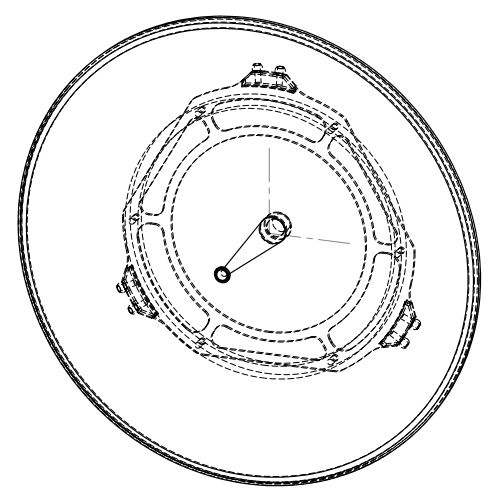
\includegraphics[width=8cm]{plat_D.JPG}
    \caption{Plataforma móvil.}
    \label{fig: cad platform}
\end{figure}

\begin{table}[hb!]
 \begin{center}
\begin{tabular}{lclc}
 Masa & $  115.53766 \ [kg]$ & $r_{cm}$ &  $[0; 0; 0.11145]^T \ [m]$ \\
 \hline
 & & & $[g/mm^2]$\\
 \hline
 $ I_x $ & $ [1 \ 0 \ 0]^T $ & $ P_x $ & 7246289714.88\\
 $ I_y $ & $ [0 \ 1 \ 0]^T $ & $ P_y $ & 7246289714.88\\
 $ I_z $ & $ [0 \ 0 \ 1]^T $ & $ P_z $ & 13887070726.86
\end{tabular}
\end{center}
\caption{Datos de inercia de la plataforma móvil.}
\label{tab: inertia table platform}
\end{table}


\subsection{Base}
\begin{figure}[htb!]
    \centering
    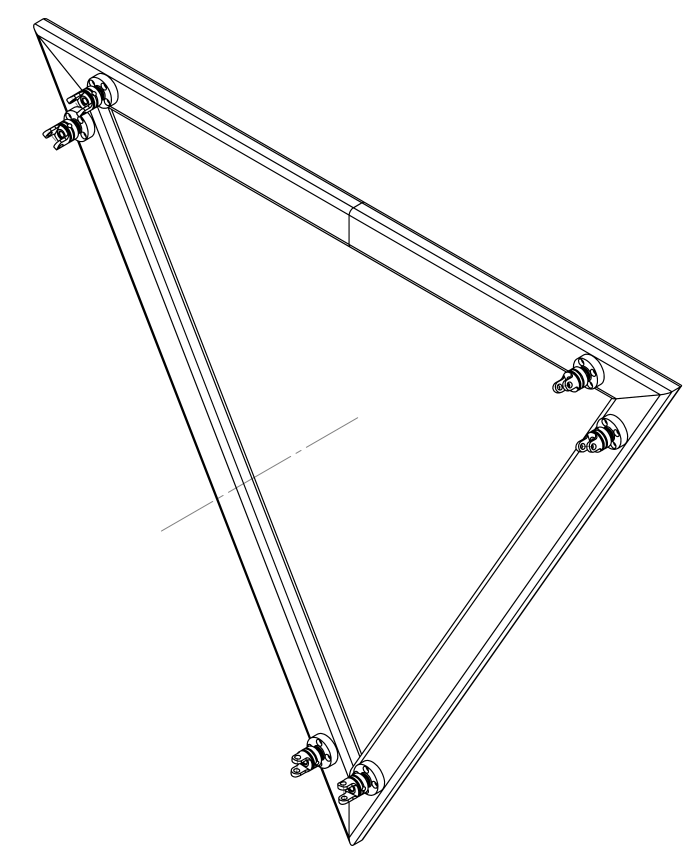
\includegraphics[width=8cm]{BASE.png}
    \caption{Base del robot.}
    \label{fig: cad base}
\end{figure}
% Px = convertGramMM2toKgM2 * 348997674.08;
% Py = convertGramMM2toKgM2 * 349004086.28;
% Pz = convertGramMM2toKgM2 * 696714510.70;
% 
% Ix = [0.73; -0.68; 0];
% Iy = [0.68; 0.73; 0];
% Iz = [0; 0; 1.0];

\begin{table}[hb!]
 \begin{center}
\begin{tabular}{lclc}
 Masa & $ 5.44739\ [kg]$ & $r_{cm}$ &  $[0; 0; 0.00048]^T \ [m]$ \\
 \hline
 & & & $[g/mm^2]$\\
 \hline
 $ I_x $ & $ [0.73\ -0.68\ 0]^T $ & $ P_x $ & 348997674.08\\
 $ I_y $ & $ [0.68\ 0.73\ 0]^T $ & $ P_y $ & 349004086.28\\
 $ I_z $ & $ [0 \ 0 \ 1]^T $ & $ P_z $ & 696714510.70
\end{tabular}
\end{center}
\caption{Datos de inercia de la base.}
\label{tab: inertia table base}
\end{table}

\subsection{Actuador prismático con motor}

\begin{figure}[htb!]
    \centering
    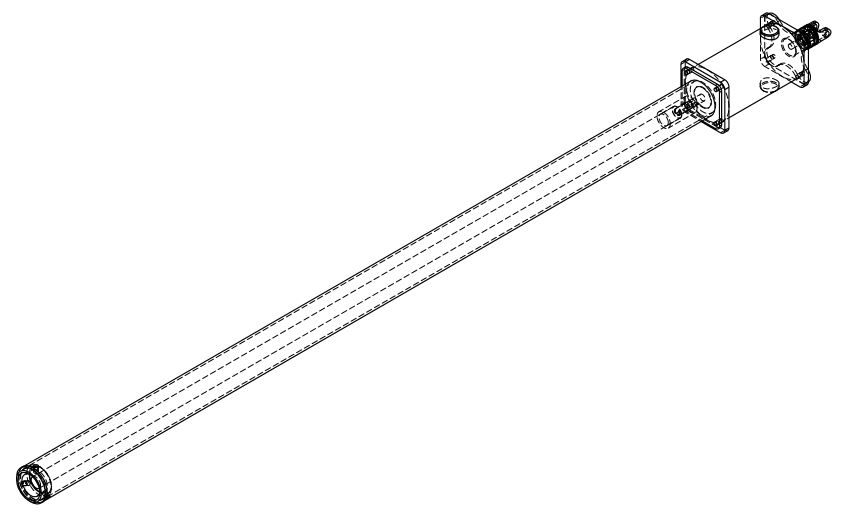
\includegraphics[width=8cm]{ACTUATOR.JPG}
    \caption{Actuador prismático.}
    \label{fig: cad motor}
\end{figure}

\begin{table}[hb!]
 \begin{center}
\begin{tabular}{lclc}


% Px = convertGramMM2toKgM2 * 2079848.97;
% Py = convertGramMM2toKgM2 * 703671034.55;
% Pz = convertGramMM2toKgM2 * 703687095.26;
% 
% Ix = [0; 0; 1];
% Iy = [0; -1; 0];
% Iz = [1; 0; 0];


 Masa & $ 5.48131 \ [kg]$ & $r_{cm}$ & $[0; 0; 0.47139]^T \ [m]$ \\
 \hline
 & & & $[g/mm^2]$\\
 \hline
 $ I_x $ & $ [0 \ 0 \ 1]^T $ & $ P_x $ & 2079848.97\\
 $ I_y $ & $ [0 \ -1 \ 0]^T $ & $ P_y $ & 703671034.55\\
 $ I_z $ & $ [1 \ 0 \ 0]^T $ & $ P_z $ & 703687095.26
\end{tabular}
\end{center}
\caption{Datos de inercia del actuador con motor.}
\label{tab: inertia table motor}
\end{table}

\subsection{Vástago con junta esférica}

\begin{figure}[htb!]
    \centering
    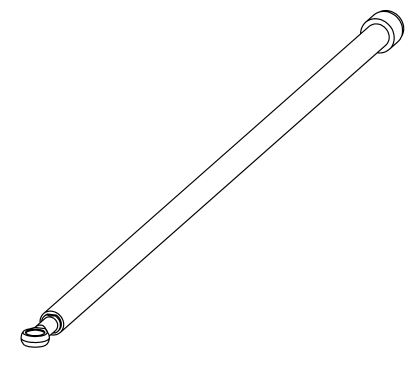
\includegraphics[width=8cm]{vastago_D.JPG}
    \caption{Vástago con junta esférica.}
    \label{fig:my_label}
\end{figure}

\begin{table}[hb!]
 \begin{center}
\begin{tabular}{lclc}


% Px = convertGramMM2toKgM2 * 297124.48;
% Py = convertGramMM2toKgM2 * 205340128.62;
% Pz = convertGramMM2toKgM2 * 205340128.62;
% 
% Ix = [0; 0; 1];
% Iy = [0.71; -0.71; 0];
% Iz = [0.71; 0.71; 0];

 Masa & $ 2.25414\ [kg]$ & $r_{cm}$ & $[0.00001; 0; -0.53696]^T \ [m]$  \\
 \hline
 & & & $[g/mm^2]$\\
 \hline
 $ I_x $ & $ [0 \ 0 \ 1]^T $ & $ P_x $ & 297124.48\\
 $ I_y $ & $ [0.71 \ -0.71 \ 0]^T $ & $ P_y $ & 205340128.62\\
 $ I_z $ & $ [0.71 \ 0.71 \ 0]^T $ & $ P_z $ & 205340128.62
\end{tabular}
\end{center}
\caption{Datos de inercia del vástago con junta esférica.}
\label{tab: inertia table joint}
\end{table}
